\documentclass{article}
\usepackage{listings}
\usepackage{graphicx}
\title{FWC RTL ASSIGNMENT-2}
\author{ALAVALA CHINNAPA REDDY}
\date{\today}
\begin{document}
\maketitle
\section{Module Code}
\begin{lstlisting}
`timescale 1ns / 1ps
module fib_gen (
 input wire reset, // External reset from switch
 input wire CLK // On Board oscillator clock
);
reg [15:0] fib_number;
reg [15:0] prev;
reg [4:0] addr_w;
reg write;
wire [15:0] ila_rv;
wire [4:0] ila_ra;
wire rsta_busy;
wire rstb_busy;
wire clk_wiz_locked;
wire clk_ph1;
wire clk_ph2;
wire fib_gen_en;

assign fib_gen_en = clk_wiz_locked & ~rsta_busy & ~rstb_busy;

assign ila_ra = addr_w- 1;

always @(posedge clk_ph1 or posedge reset)
begin
 if(reset)
 begin
 fib_number <= 0;
 prev <= 1;
 addr_w<= 6'd31;
 write <= 1;
 end
 else if(fib_gen_en)
 begin
 fib_number <= (fib_number+prev >= fib_number) ? fib_number+prev :1;

 prev <= (fib_number+prev>= fib_number) ? fib_number : 0;

 addr_w <= addr_w + 1;
 write <= 1;
 end
end

blk_mem_gen_0 fibonacci_memory (
 .clka(clk_ph2), // input wire clka
 .rsta(reset), // input wire rsta
 .ena(1'b1), // input wire ena
 .wea(write), // input wire [0 : 0] wea
 .addra(addr_w), // input wire [4 : 0] addra
 .dina(fib_number), // input wire [15 : 0] dina
 .douta(), // output wire [15 : 0] douta
 .clkb(clk_ph2), // input wire clkb
 .rstb(reset), // input wire rstb
 .enb(1'b1), // input wire enb
 .web(1'b0), // input wire [0 : 0] web
 .addrb(ila_read_address), // input wire [4 : 0] addrb
 .dinb(), // input wire [15 : 0] dinb
 .doutb(ila_rv), // output wire [15 : 0] doutb
 .rsta_busy(rsta_busy), // output wire rsta_busy
 .rstb_busy(rstb_busy) // output wire rstb_busy
);

clk_wiz_1 fibonacci_clk
   (
    // Clock out ports
    .clk_out1(clk_ph1),     // output clk_out1
.clk_out2(clk_ph2),     // output clk_out2
    // Status and control signals
    .reset(reset), // input reset
    .locked(clk_wiz_locked),       // output locked
   // Clock in ports
    .clk_in1(CLK)
    );   
 
// ILA:
ila_0 fibonacci_debug (
.clk(CLK), // input wire clk - 100 MHz
.probe0(fib_gen_en), // input wire [0:0] probe0
.probe1(clk_ph2), // input wire [0:0] probe1
.probe2(ila_read_address), // input wire [4:0] probe2
.probe3(ila_rv) // input wire [15:0] probe3
);
endmodule





    \end{lstlisting}




\section{Testbench Code}
\begin{lstlisting}
`timescale 10ns / 1ns
module fibonacci_generator_tb;
reg reset, clk;
wire [15:0] number;
wire [15:0] read_number;
wire [4:0] read_address;
wire fib_gen_en;
wire ph1, ph2;
fib_gen UUT(
 .reset(reset),
 .CLK(clk)
);
assign fib_gen_en = UUT.fib_gen_en;
assign number = UUT.fib_number;
assign read_number = UUT.ila_rv;
assign read_address = UUT.ila_ra;
assign ph1 = UUT.clk_ph1;
assign ph2 = UUT.clk_ph2;
initial begin
 clk = 1'b0;
 forever #1 clk = ~clk;
end
initial begin
 reset = 1;
 #15 reset = 0;
 #400 reset = 1;
 #20 reset = 0;
 #400
 $finish;
end
endmodule
\end{lstlisting}
\section{Timing Diagram-simulation}
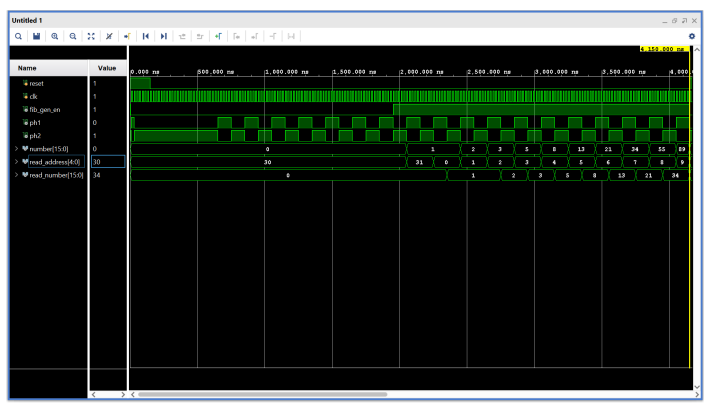
\includegraphics[width=1\columnwidth]{figs/4.jpeg}
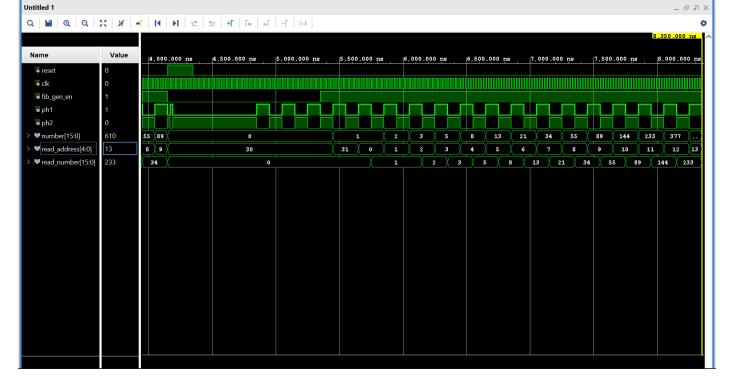
\includegraphics[width=1\columnwidth]{figs/5.jpeg}
\section{Timing Diagram-ILA}
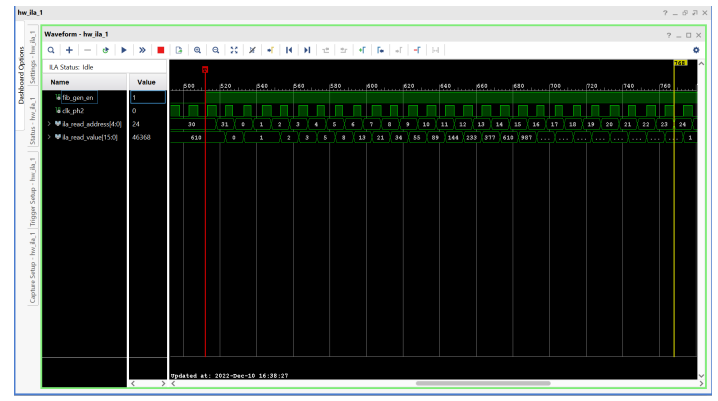
\includegraphics[width=1\columnwidth]{figs/6.jpeg}
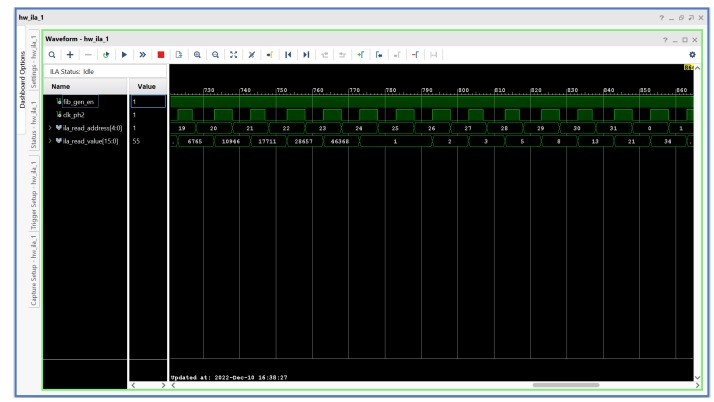
\includegraphics[width=1\columnwidth]{figs/7.jpeg}
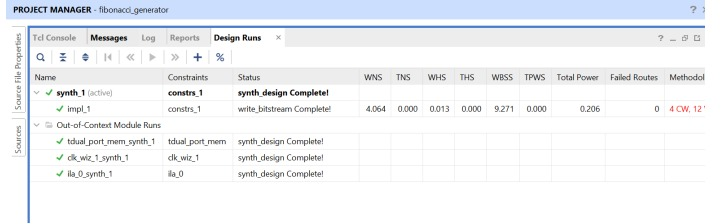
\includegraphics[width=1\columnwidth]{figs/8.jpeg}

\section{Constraints}
\begin{lstlisting}

## This file is a general .xdc for the Nexys A7-100T
## To use it in a project:
## - uncomment the lines corresponding to used pins
## - rename the used ports (in each line, after get_ports) according to the top level
##signal names in the project
## Clock signal
set_property -dict { PACKAGE_PIN E3 IOSTANDARD LVCMOS33 } [get_ports { CLK}];
#IO_L12P_T1_MRCC_35 Sch=clk100mhz
create_clock -add -name sys_clk_pin -period 10.00 -waveform {0 5} [get_ports
{CLK100MHZ}];
## Reset pin
set_property -dict { PACKAGE_PIN J15 IOSTANDARD LVCMOS33 } [get_ports { reset }];
#IO_L18P_T2_A24_15 Sch=led[0]
## Do not analyze any timing paths between clk_out2_clk_wiz_1 and sys_clk_pin ( Large
##path delay causes negative WHS )
## This path occurs only at ILA inputs ( violation of WHS is not critical since ILA
##used for signal monitoring )
set_false_path -from [get_clocks clk_out2_clk_wiz_1] -to [get_clocks sys_clk_pin];


\end{lstlisting}
\end{document}

